\documentclass{article}
\usepackage{graphicx}
\usepackage[dvipsnames,table]{xcolor}
\usepackage[utf8]{inputenc}
\usepackage{siunitx}
\usepackage[american,siunitx]{circuitikz}
\usepackage{amsmath}
\usepackage{svg}
\usepackage{booktabs}
\usepackage{float}
\usepackage{xparse, xfp}
\usepackage{multirow}
\usepackage{tikz}
\usepackage{karnaugh-map}
\usepackage{pdfpages}
\usepackage{hyperref}
\hypersetup{
    colorlinks=true,
    linkcolor=blue,
    filecolor=magenta,      
    urlcolor=cyan,
}
\usepackage{caption} 

\makeatletter
\ctikzset{lx/.code args={#1 and #2}{ 
  \pgfkeys{/tikz/circuitikz/bipole/label/name=\parbox{1cm}{\centering #1  \\ #2}}
    \ctikzsetvalof{bipole/label/unit}{}
    \ifpgf@circ@siunitx 
        \pgf@circ@handleSI{#2}
        \ifpgf@circ@siunitx@res 
            \edef\pgf@temp{\pgf@circ@handleSI@val}
            \pgfkeyslet{/tikz/circuitikz/bipole/label/name}{\pgf@temp}
            \edef\pgf@temp{\pgf@circ@handleSI@unit}
            \pgfkeyslet{/tikz/circuitikz/bipole/label/unit}{\pgf@temp}
        \else
        \fi
    \else
    \fi
}}

\ctikzset{lx^/.style args={#1 and #2}{ 
    lx=#2 and #1,
    \circuitikzbasekey/bipole/label/position=90 } 
}

\ctikzset{lx_/.style args={#1 and #2}{ 
    lx=#1 and #2,
    \circuitikzbasekey/bipole/label/position=-90 } 
}
\makeatother

\captionsetup[table]{skip=10pt}

\usetikzlibrary{calc}
%\usepackage[landscape]{geometry}
\renewcommand{\thesubsection}{\thesection.\alph{subsection}}
\newcommand{\equal}{=}
\newcommand{\greyrule}{\arrayrulecolor{black!30}\midrule\arrayrulecolor{black}}
\makeatletter
\newcommand\currcoor{\the\tikz@lastxsaved,\the\tikz@lastysaved}
\makeatother
\newcolumntype{:}{@{\hskip\tabcolsep\color{black!30}\vrule\hskip\tabcolsep}}

\ExplSyntaxOn
\NewExpandableDocumentCommand \groupify { O{\,\allowbreak} m m }
  { \jakob_groupify:nnn {#1} {#2} {#3} }
\cs_new:Npn \jakob_groupify:nnn #1 #2 #3
  { \__jakob_groupify_loop:nnw { 1 } {#2} #3 \q_recursion_tail {#1} \q_recursion_stop }
\cs_new:Npn \__jakob_groupify_loop:nnw #1 #2 #3
  {
    \quark_if_recursion_tail_stop:n {#3}
    \exp_not:n {#3}
    \int_compare:nNnTF {#1} = {#2}
      { \__jakob_groupify_sep:n }
      { \exp_args:Nf \__jakob_groupify_loop:nnw { \int_eval:n { #1+1 } } }
          {#2}
  }
\cs_new:Npn \__jakob_groupify_sep:n #1 #2 \q_recursion_tail #3
  {
    \tl_if_empty:nF {#2} { \exp_not:n {#3} }
    \__jakob_groupify_loop:nnw { 1 } {#1}
    #2 \q_recursion_tail {#3}
  }
\ExplSyntaxOff

\title{ECE 2200L\\Introduction to Microelectronics Circuits Laboratory\\\,\\Experiment 10\\Current-Voltage Characteristics of the Junction Field Effect Transistor\\\,\\Report}
\author{Choi Tim Antony Yung}
\date{November 25, 2020}
\begin{document}
\maketitle

\thispagestyle{empty}
\setcounter{page}{0}

\newpage

\section*{Objective}
To study the relationships between the terminal currents and terminal voltages in the Junction Field Effect Transistor (JFET), a useful 3-terminal device that has structure and characteristics very similar to Metal Semiconductor Field Effect Transistors (MESFET) used in high-speed III-V compound-based semiconductor devices.
\section*{Result}

\begin{figure}[H]
  \centering
  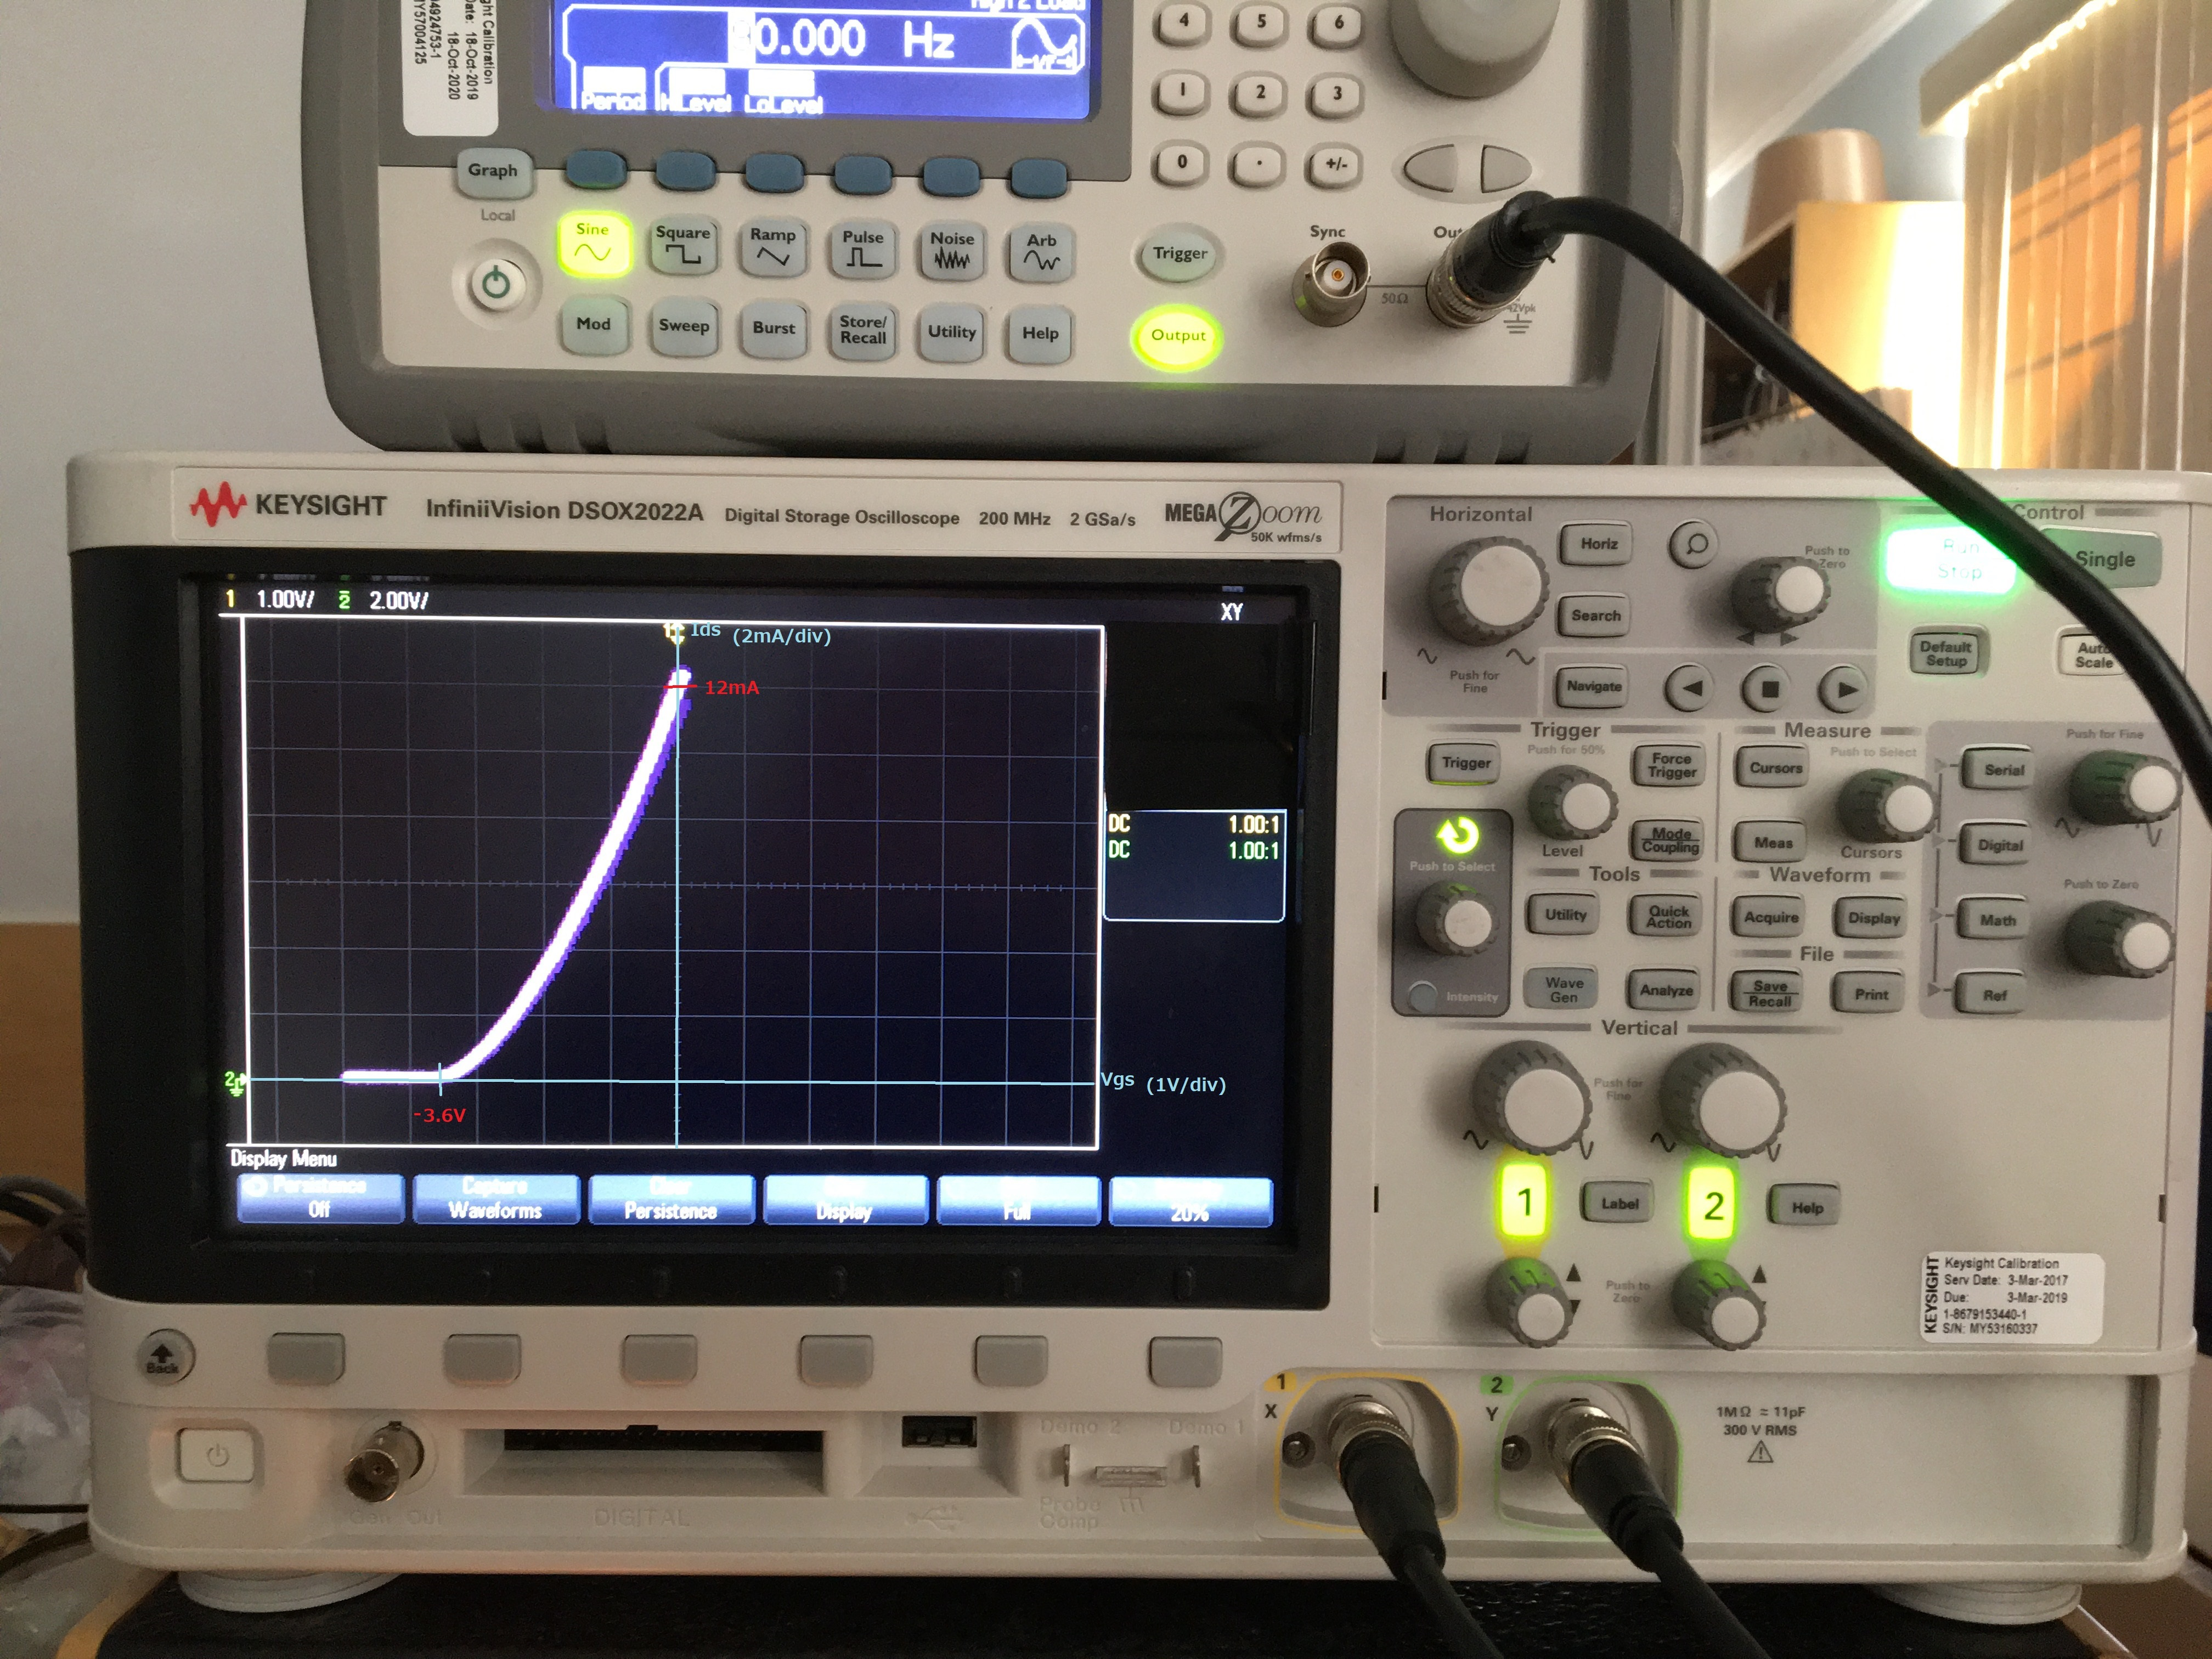
\includegraphics[width=\textwidth]{ECE2200L_Lab10_IVgs.JPG}
  \caption{$I_{DS}$ vs. $V_{GS}$ plot from oscilloscope}
  \label{fig:ivgs}
\end{figure}

Figure \ref{fig:ivgs} shows $I_{DS}$ vs. $V_{GS}$ plot assuming $\lambda = 0$, we can thus derive $I_{DSS}$ as follow,
$$I_D = I_{DSS} \left(1-\frac{V_{GS}}{V_p}\right)^2(1+\lambda V_{DS})$$
$$I_D(V_{GS} = 0, \lambda = 0) = I_{DSS} \left(1-\frac{0}{V_p}\right)^2(1+0 V_{DS})$$
$$I_D(V_{GS} = 0, \lambda = 0) = I_{DSS} = \SI{12}{\milli\ampere}$$
Pinch-off voltage $V_p$ is the threshold value of $V_{GS}$ below which the transistor turns off, which we can derived from the plot as the maximum value of $V_{GS}$ that $I_{DS}$ stays 0, which is $V_p = \SI{-3.6}{\volt}$

\begin{figure}[H]
  \centering
  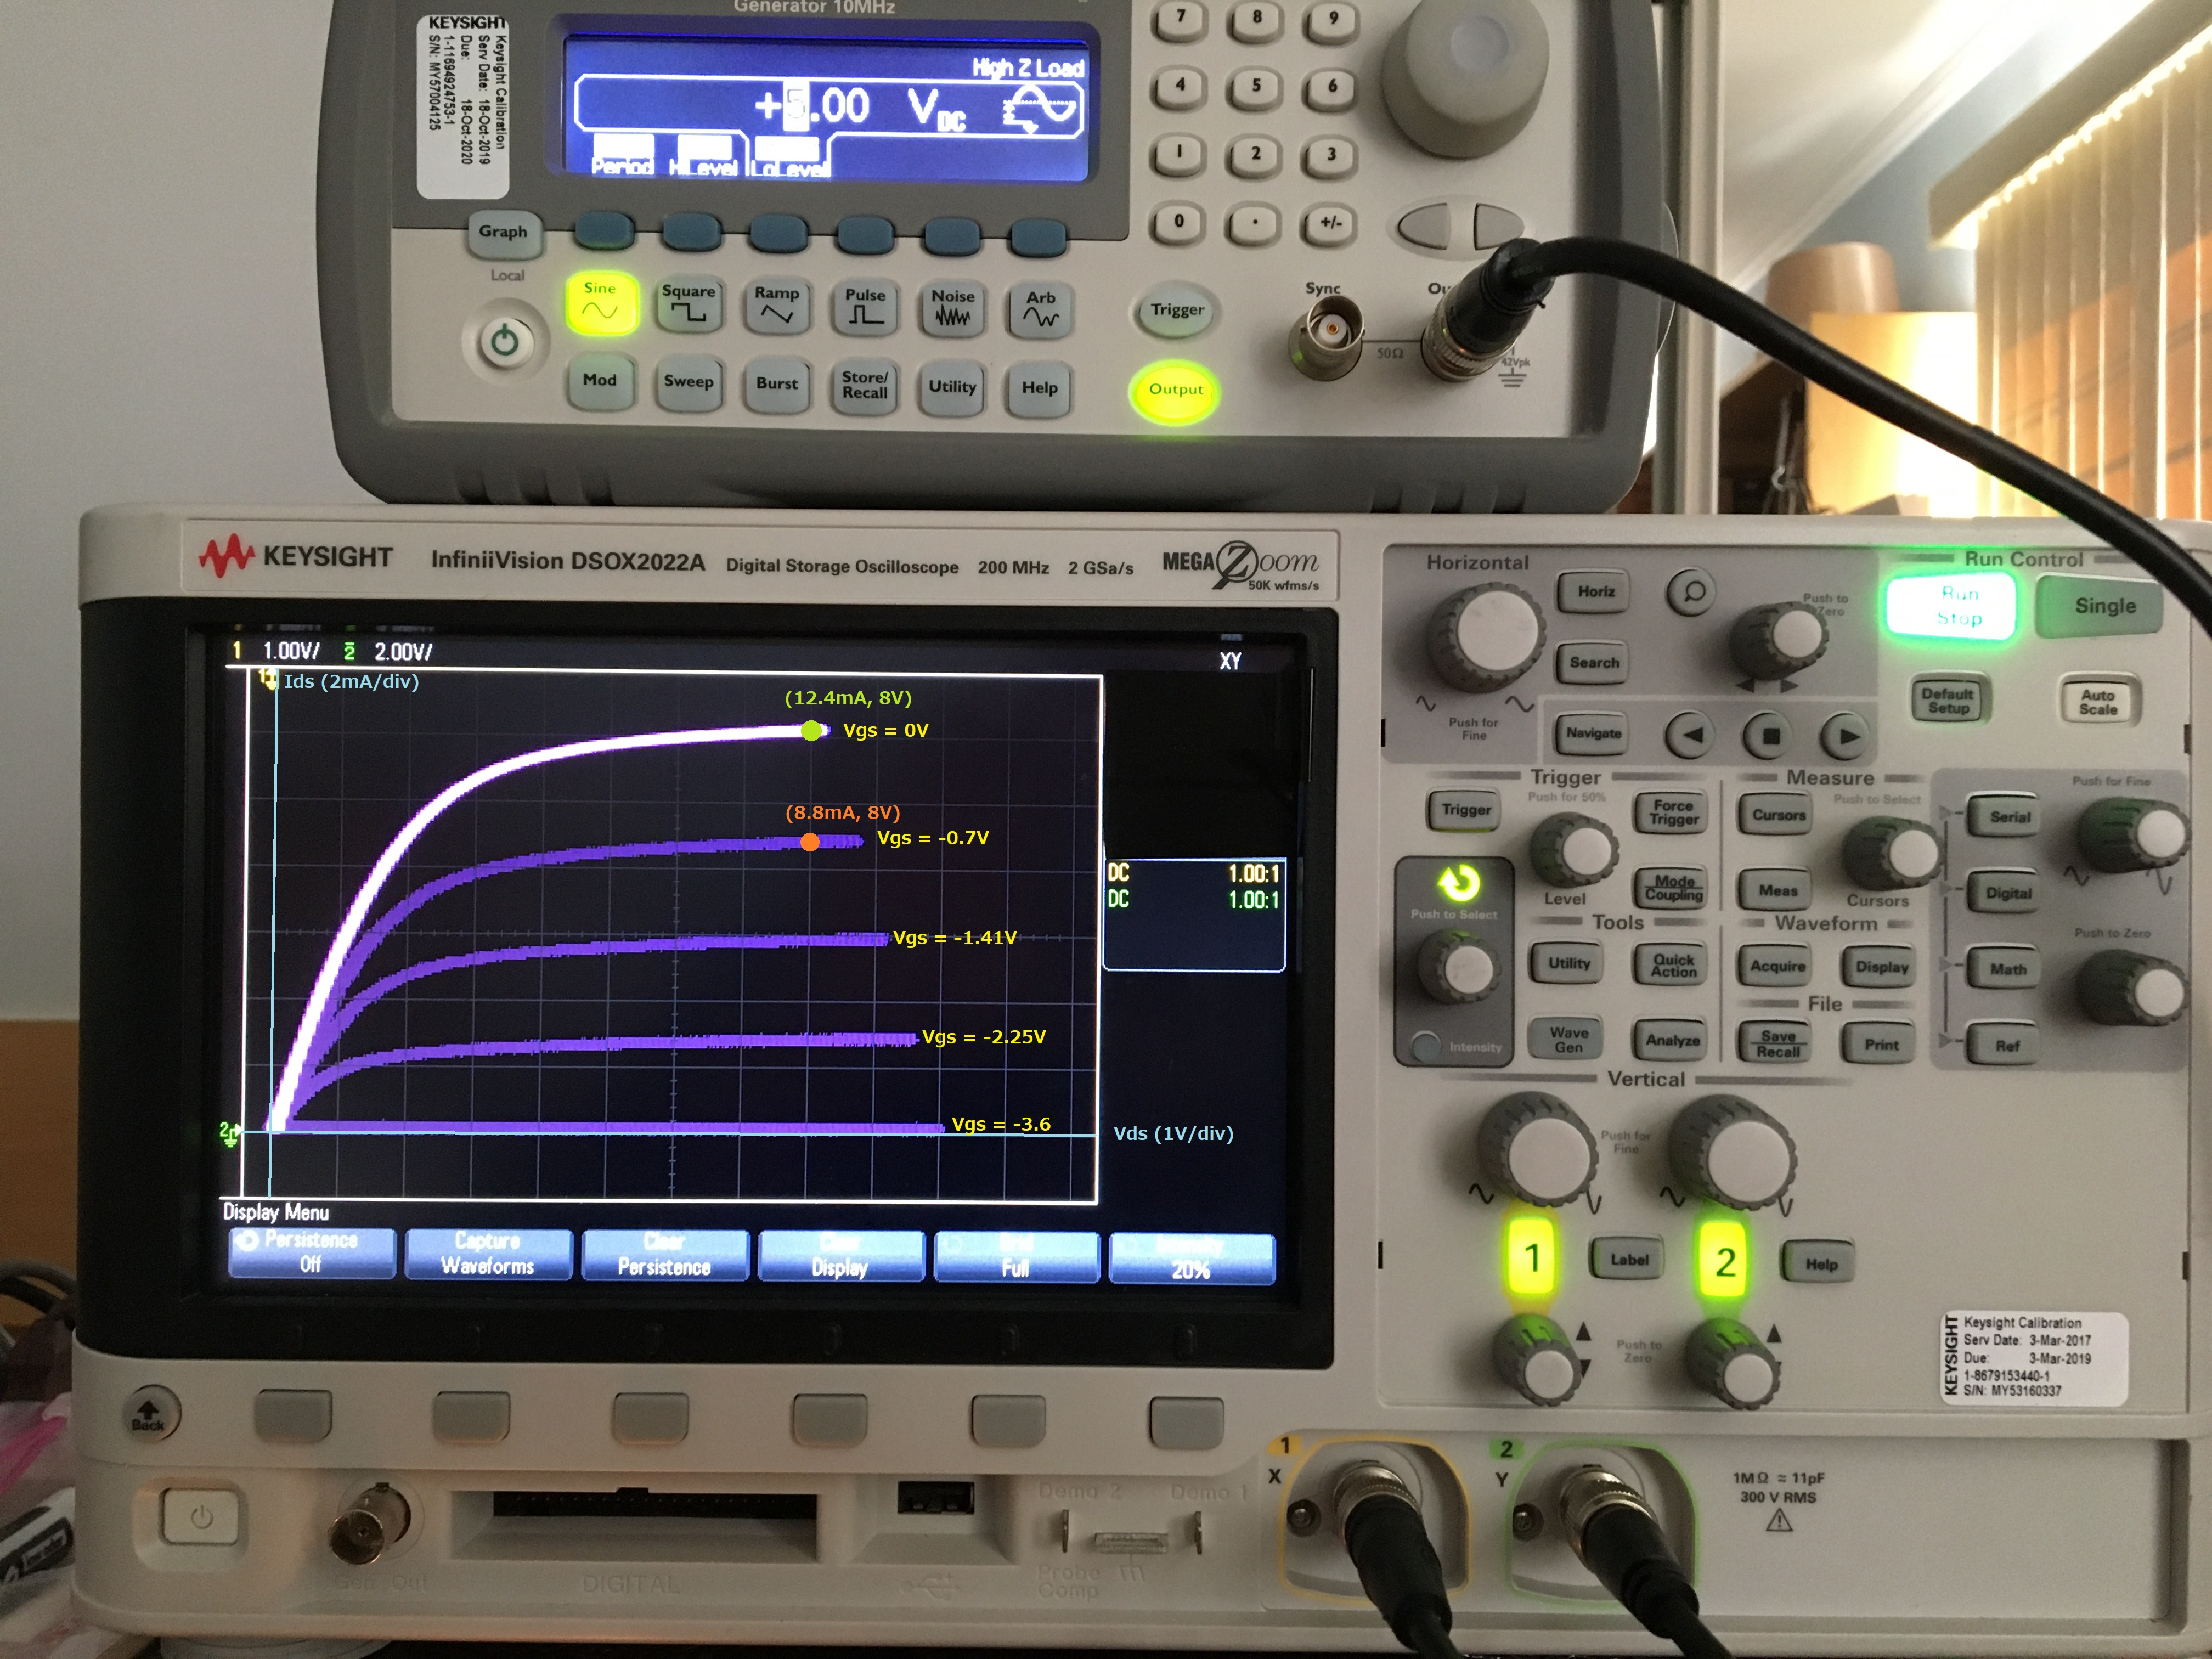
\includegraphics[width=\textwidth]{ECE2200L_Lab10_IVds.JPG}
  \caption{$I_{DS}$ vs. $V_{DS}$ plot from oscilloscope with varying $V_{GS}$ values}
  \label{fig:ivds}
\end{figure}
$\lambda$ can be approximated by extending the plot at saturation region as a line to its x-intercept.
Using (12.4mA,8V) and (12mA,6.5V), we can approximate $V_A$ to be \SI{38.5}{volt} and $\lambda$ to be \SI{0.026}{\volt}$^{-1}$

Figure \ref{fig:ivds} shows $I_{DS}$ vs. $V_{DS}$ plot from oscilloscope with varying $V_{GS}$ values.
From this plot we can then derive $I_{DSS}$ and $V_p$ assuming lambda is \SI{0.026}{\volt}$^{-1}$.
$$I_D = I_{DSS} \left(1-\frac{V_{GS}}{V_p}\right)^2(1+\lambda V_{DS})$$
$$I_D = I_{DSS} \left(1-\frac{V_{GS}}{V_p}\right)^2(1+0.026 V_{DS})$$
$$\SI{12.4}{\milli\ampere} = I_{DSS} \left(1-\frac{0}{V_p}\right)^2(1+0.026 (8))$$
$$I_{DSS} = \SI{10.3}{\milli\ampere}$$
$$\SI{8.8}{\milli\ampere} =  \SI{12.4}{\milli\ampere}\left(1-\frac{-0.7}{V_p}\right)^2(1+0.026 (8))$$
$$\sqrt{\frac{\SI{8.8}{\milli\ampere}}{(1.208)\SI{12.4}{\milli\ampere}}}=1-\frac{-0.7}{V_p}$$
$$V_p= \frac{-0.7}{1-\sqrt{\frac{\SI{8.8}{\milli\ampere}}{(1.208)\SI{12.4}{\milli\ampere}}}}$$
$$V_p = -\SI{3.00}{\volt}$$

\section*{Conclusion}
As demonstrated above, the values of $I_{DSS}$ and $V_p$ obtained from the above two graph are different from each other which is likely a result of the diffrerent value of $\lambda$ used to obtain the values.
\end{document}
